\setcounter{equation}{0}
Будем рассматривать уравнение второго порядка:
\begin{equation}\label{lin_sec}
    y'' + a(x)y'+b(x)y=0
\end{equation}
где $a(x),b(x)$ -- действительно-значные функции, заданные на $I\subseteq \R$ и $a(x) \in C^1(I), \; b(x)\in C(I)$.
\bigbreak
\noindent \Def  Решение называется \textit{нетривиальным} (на $I$), если оно не равно нулю хотя бы в одной точке $x_0 \in I$.
\\
\Def Решение, имеющее более одного нуля на $I$, называется \textit{колеблющимся}.
\\
\Def Значение $x_0$ называется \textit{простым нулём} функции $f(x)$, определенной и дифференцируемой в точке $x_0$, если $f(x_0) = 0$ и $f'(x_0)\neq 0$. Если производная равна 0, то такое значение называется \textit{кратным нулём}.
\bigbreak
Выполним в (\ref{lin_sec}) замену $y(x) = u(x)\cdot z(x)$, так как хотим понизить порядок. Приэтом $z(x)$ -- будет неизвестной функцией, а $u(x)$ -- подберем так, как нам будет нужно:
\begin{gather*}
    y' = u'z + uz' \\
    y'' = u''z + 2u'z' + uz''
\end{gather*}
Подставляем в (\ref{lin_sec}):
\begin{equation*}
    uz'' + \underbrace{(2u'+au)}_{\text{хотим } =0}z'+(u''+au'+bu)z=0
\end{equation*}
Возьмем $u(x)=\exp\Big[-\frac{1}{2}\int\limits_{x_0}^{x}a(t)dt\Big]$ -- решение уравнения $2u'+au=0$. Заметим, что $u(x)$ в 0 никогда не обращается. Подставим $u(x)$ в полученное выше уравнение:
\begin{equation}\label{simpl}
    z''(x)+q(x)z=0, \qquad \quad q(x)=\frac{u''+au'+bu}{u}
\end{equation}
Полученное уравнение называется \textit{приведённым}. (К такому виду уравнение можно привести всегда.)
\bigbreak
\textbf{Лемма 1:} Если $z(x)$ -- нетривиальное решение приведённого уравнения (\ref{simpl}), то каждый его
нуль на промежутке $I$ является простым.

\Proof Пусть это не так, т.е. $x_0 \in I$ -- кратный нуль:
\begin{equation*}
    \begin{cases}
    z''(x)+q(x)z=0\\
    z(x_0)=0\\
    z'(x_0)=0
    \end{cases}
\end{equation*}
Решение полученной ЗК единственно. Более того, оно равно нулю на всём $I$ --
противоречие.\;\; \EndProof
\bigbreak
\textbf{Лемма 2:} Нули любого нетривиального решения (\ref{simpl}) не имеют конечной предельной точки на $I$.

\Proof Пусть это не так, т.е. существует $\{x_n\}$ -- последовательность нулей $z(x)$, которая сходится к $x_0 \in I$. В силу непрерывности $z(x)$ имеем $\lim\limits_{x\to x_0}z(x) = z(x_0)= \lim\limits_{n\to\infty}z(x_n) = 0$. \newline Значит $x_0$ -- тоже нуль функци $z(x)$. Далее, по определению
\begin{equation*}
    z'(x_0)=\lim\limits_{n\to\infty}\frac{z(x_n)-z(x_0)}{x_n-x_0}=0
\end{equation*}
Таким образом, $x_0$ оказался кратным нулём, что противоречит лемме 1. \;\EndProof
\bigbreak
\textbf{Следствие:} Любое нетривиальное на $[\alpha, \beta] \subseteq I$ решение уравнения (\ref{simpl}) имеет не более конечного числа нулей на этом отрезке.

\Proof От противного. Если их счетное число, то для них получаем предельную точку нулей (теореме по Больцано-Вейерштрасса), отсюда противоречие лемме 2. \;\EndProof
\newpage

\textbf{Теорма (Штурма):} Рассмотрим $y''+q(x)y=0$ и $z''+Q(x)z=0$ -- уравнения (3) и (4) соответсвенно.
\newline Пусть $\forall x\in I \;\; q(x)\leqslant Q(x)$ и пусть $y(x)$, $z(x)$ --
нетривиальные решения уравнений (3) и (4) соответсвенно.  Если $x_1 \leqslant x_2$ -- последовательные нули $y(x)$, то 
\begin{figure}[h]
    \hspace{-4ex}
    \begin{minipage}[h]{0.5\linewidth}
    \vspace{-2ex}
    \begin{itemize}
        \item либо $z(x_1) = z(x_2) = 0$
        \item либо существует хотя бы одна \newline точка $x_0 \in (x_1, x_2)$, для которого \newline выполнено $z(x_0) = 0$.
    \end{itemize}
    \end{minipage}
    \hspace{-4ex}
    \begin{minipage}[h]{0.5\linewidth}
    \vspace{-2ex}
    \begin{center}
    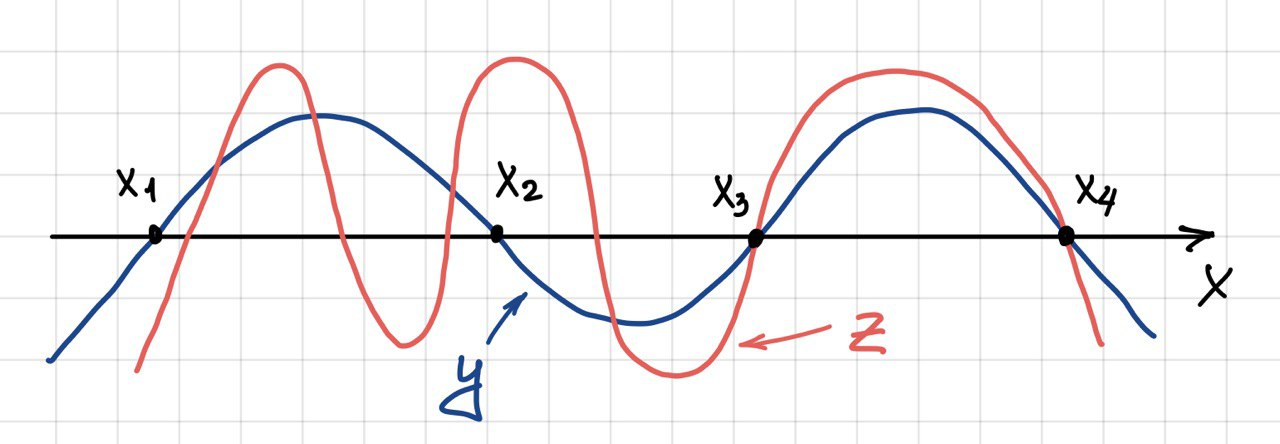
\includegraphics[width=1\linewidth]{images/shturma.jpg}
\end{center}
    \end{minipage}
\end{figure}
\\
\Proof Будем действовать от противного: предположим, что $z(x) \neq 0$ на $(x_1, x_2)$, т.е. например, $z(x) > 0$.
\newline Без потери общности предположим, что $y(x) > 0$ на $(x_1,x_2)$. Из условия теоремы: $y(x_1)=y(x_2)=0$. Тогда
\begin{equation*}
    y'(x_1)=\lim\limits_{x\to x_1+0}\frac{y(x)-y(x_1)}{x-x_1}\geqslant 0
    \qquad \qquad y'(x_2)=\lim\limits_{x\to x_2-0}\frac{y(x)-y(x_2)}{x-x_2}\leqslant 0
\end{equation*}
Но поскольку $x_1,x_2$ -- простые нули (т.к. решения нетривиальные), то $y'(x_1)>0$ и $y'(x_2)<0$.
\\
Посчитаем $(3)\cdot z - (4) \cdot y$:
\setcounter{equation}{4}
\begin{equation}\label{prom}
    y''z - z''y = (Q-q)yz
\end{equation}
Вычислим интеграл левой части:
\begin{align*}
    \int\limits_{x_1}^{x_2}(y''z-z''y)dx &= \int\limits_{x_1}^{x_2}zdy' - \int\limits_{x_1}^{x_2}ydz' = \\ &=
    (zy')\Big|_{x_1}^{x_2}-\int\limits_{x_1}^{x_2}y'dz \;-\; (yz')\Big|_{x_1}^{x_2} + \int\limits_{x_1}^{x_2}z'dy = 
\end{align*}
При этом верно: $dz=z'dx$ и $dy=y'dx$. Поэтому полученные интегралы совпадают и сокращаются. 
\begin{align*}
    = (zy')\Big|_{x_1}^{x_2} - \cancelto{0}{(yz')\Big|_{x_1}^{x_2}} \text{\qquad сокращается, так как $y(x_1)=y(x_2)=0$}
\end{align*}
Тогда (\ref{prom}) принимает вид:
\begin{equation}\label{final}
    z(x_2)y'(x_2)-z(x_1)y'(x_1) = \int\limits_{x_1}^{x_2}\underbrace{(Q-q)yz}_{\geqslant0}\,dx \geqslant 0
\end{equation}
Далее возможны следующие варианты:
\begin{equation*}
    \text{$\bullet$ \;$z > 0$ на $[x_1, x_2]$ \qquad\; $\bullet$ \;$z > 0$ на $[x_1, x_2)$, и $z(x_2) = 0$ \qquad\; $\bullet$\; $z > 0$ на $(x_1, x_2]$, и $z(x_1) = 0$ }
\end{equation*}
Заметим, что левая часть (\ref{final}) во всех случаях отрицательна $\Rightarrow$ противоречие.\; \EndProof
\bigbreak
\noindent \textbf{Следствие 1:} Если $q(x) \leqslant 0$, то любое нетривиальное решение уравнения $y''+q(x)y = 0$ имеет не более одного нуля.
\\
\Proof Предположим, что есть нетривиальное решение $y(x)$, у которого есть 2 последовательных нуля.
\\
Тогда пусть $Q(x)\equiv0$, то есть $z''+0\cdot z = 0 \;\; \Rightarrow \;\; z = ax + b \neq 0$. \newline Возьмем $z\equiv 5$. Но эта функция не имеет ни одного нуля $\;\Rightarrow\;$ противоречие с теоремой Штурма. \;\EndProof
\bigbreak
\noindent \textbf{Следствие 2:} Пусть $y_1(x)$ и $y_2(x)$ — линейно независимые решения уравнения $y'' +q(x) y = 0$. \newlineЕсли $x_1$ и $x_2$ — последовательные нули $y_1$, то между ними имеется ровно один
нуль $y_2$.
\\
\Proof Положим $q(x) \equiv Q(x)$. Заметим, что $y_1$ и $y_2$ не обращаются одновременно в нуль в $x_1$ и $x_2$ (ввиду линейной независимости). Если предположить, что между
$x_1$ и $x_2$ лежит \underline{хотя бы два} нуля $y_2$, то аналогичным образом получается, что между этими нулями есть ещё хотя бы один нуль $y_1$. \; \EndProof
\bigbreak
\noindent \textbf{Следствие 3:} Если некоторое нетривиальное решение уравнения $y'' + q(x) y = 0$ имеет
бесконечно много нулей, то и любое другое решение также имеет бесконечно много нулей.